\documentclass[11pt,french]{article}
\usepackage{mathrsfs}
\usepackage{eurosym}
\usepackage{amsmath,amssymb,amsfonts}

\usepackage[T1]{fontenc}
\usepackage[french]{babel}

\usepackage[utf8]{inputenc}
\usepackage{aeguill}
\usepackage{hyperref}
\usepackage{array}
\makeatletter
%%%%%%%%%%%%%%%%%%%%%%%%%%%%%% Textclass specific LaTeX commands.
\usepackage{framed}
\usepackage[framed]{ntheorem}
\newframedtheorem{theoreme}{Théorème}

%definition
\def\theoremframecommand#1{\vrule\hspace{6pt}\hbox{#1}}
\setlength\theorempreskipamount{0pt}%
\setlength\theorempostskipamount{0pt}%
\newshadedtheorem{definition}{\protect\definitionname}
\theoremprework{%
    \setlength\theorempreskipamount{\topsep}%
    \setlength\theorempostskipamount{\topsep}%
}
\theoremstyle{plain}
\theorembodyfont{\upshape}
\newtheorem*{remarque}{Remarque}
\newframedtheorem{propriete}{Propriété}
\newtheorem*{notation}{Notation}
\newtheorem*{proof}{Preuve}
\newtheorem*{exemple}{Exemple}
\newtheorem{exercice}{Exercice}

% Définition des environnements pour les théorèmes, proposition, etc...

\providecommand{\definitionname}{Définition}
\providecommand{\definitionname}{exemple}
\providecommand{\definitionname}{preuve}
\providecommand{\definitionname}{remarque}
\providecommand{\definitionname}{propriete}
\providecommand{\theoremname}{Notation}
%%%%%%%%%%%%%%%%%%%%%%%%%%%%%% User specified LaTeX commands.

\usepackage{fourier} % math & rm
\usepackage[scaled=0.875]{helvet} % ss
\usepackage[normalem]{ulem}
\usepackage{pifont}
\usepackage{pgf,tikz,pgfplots}
\pgfplotsset{compat=1.15}
\usepackage[tikz]{bclogo}
\usetikzlibrary{positioning,shapes,decorations}
\usepackage{wrapfig}
\usepackage{mathrsfs}
\usetikzlibrary{arrows}
\usepackage{multicol}

\setlength{\columnseprule}{0.5pt}
\setlength{\columnsep}{20pt}
\usepackage{smartdiagram}
\usepackage[paperwidth=210mm,paperheight=297mm]{geometry}
%\geometry{verbose,tmargin=2cm,bmargin=15mm,lmargin=2cm,rmargin=2cm,headheight=1cm,headsep=5mm,footskip=5mm}
\usepackage{fancyhdr}
\hypersetup{
            pdftitle={Algorithme de Karatsuba},
            pdfauthor={Pascal Malingrey},
            pdfkeywords={Algorithme, Karatsuba, DIU},
            pdfborder={0 0 0},
            pdfsubject={Etude Algorithme de Karatsuba},
            breaklinks=true}

\usepackage{xcolor}
\usepackage[tikz]{bclogo}
\usepackage{wrapfig}
%\usepackage{algorithm}
\usepackage[ruled,vlined]{algorithm2e}% incompatible avec algorithm
%\usepackage{algpseudocode}
\usepackage{listings,lipsum,listingsutf8}
\definecolor{codegreen}{rgb}{0.1,0.47,0.1}
\definecolor{fondjaune}{rgb}{0.99, 0.7,0.8}
\definecolor{couleurdef}{rgb}{0.99, 0.8, 0.87}
\definecolor{codegray}{rgb}{0.5,0.5,0.5}
\definecolor{codepurple}{rgb}{0.58,0,0.82}
\definecolor{backcolour}{rgb}{0.95,0.95,0.92}
\DeclareMathOperator{\lgd}{long}
\newenvironment{code}[1]{%
    \begin{bclogo}[couleur=backcolour, couleurTexte=black ,couleurBord=blue ,couleurBarre=black, ombre=false,epBord=0.9,logo=\#,arrondi=0.1]{{\bfseries #1}}%
    }%
    {%
    \end{bclogo}
}%
%---------------------------- version élève - prof
\newcommand{\ka}{\textbf{kar}}
\newboolean{Prof}

\newcommand{\cacher}[1]{
    \ifthenelse{\boolean{Prof}} % si « Professeur » est vrai,
    {#1} %les mots cachés sont en gras
    {\dashuline{\phantom{#1}}} % (else) sinon les mots sont remplacés par une ligne sur laquelle l'élève peut écrire. 
}
\newcommand{\cacherb}[1]{
    \ifthenelse{\boolean{Prof}} % si « Professeur » est vrai,
    {#1} %les mots cachés sont en gras
    {\phantom{#1}} % (else) sinon les mots sont remplacés par une ligne sur laquelle l'élève peut écrire. 
}
%-------------------------------------------------------
%\usepackage{minted}
\title{Dossier algorithme :
\\
Algorithme de Karatsuba}
\author{Pascal Malingrey}
\date{20 août 2019}
%------------------------------------------------------------
\usepackage{fancyhdr}
\pagestyle{fancy}
\lhead{\Large \title}
\rhead{DIU: Algorithme}
\setlength{\parindent}{0mm}

\AtBeginDocument{ % Nécessaire à cause de babel
\renewcommand\labelitemi{\textbullet}
\renewcommand\labelitemii{\textasteriskcentered}
\renewcommand\labelitemiii{\textperiodcentered}
}
\newcommand{\x}{\times}
\newcommand{\cd}{\centerdot}
\usepackage{xlop}


\begin{document}

\maketitle

\tableofcontents
\newpage

\section{Présentation}

\begin{bclogo}{Le problème}
Nous désirons effectuer la multiplication de deux grands entiers écrits dans une base donnée $\alpha$: la base décimale et la base binaire seront privilégiées.
\end{bclogo}
Dans la suite, la distinction sera faite entre la multiplication par $\alpha$ notée $\centerdot$ et la multiplication classique notée $\times$. La multiplication par $\alpha$ n'a pas le même coût que la multiplication classique. \\ Par exemple en binaire, il s'agit d'un décalage de bit et en décimal, l'ajout d'un 0 à la fin d'une liste si on représente le nombre par une liste.

\subsection{Exemple introductif}

Dans ce premier exemple nous allons traiter la multiplication de 57 par 34.
\subsubsection{Méthode classique}
%\opmul{57}{34}\\
$57 \times 34=(5\centerdot 10 + 7)\times (3 \centerdot10 +4 )=5\x 3 \centerdot 10^2 + (5\x4+7\x3)\cd 10+7\x4=15\cd 10^2 + 41\cd 10 + 28=1938$

Le coût de cette opération est de 4 multiplications et de trois  additions (les trois additions ne sont pas équivalentes).

\subsubsection{Réduction du nombre de multiplications}

Pour comprendre le fonctionnement, il est plus simple de travailler avec une écriture générique.
On considère deux entiers $m$ et $p$ avec $a_1,\, a_2, \, b_1$ et $b_2$ entiers inférieurs strictement à $x$.
\begin{equation}
m\x p = \overline{a_1 a_2}\x \overline{b_1 b_2} =  a_1 b_1 x^2 + \left( a_1 b_2 +a_2 b_1\right)x+a_2 b_2  \label{eqc}
\end{equation}


L'idée est de remplacer les deux produits croisés (du milieu), par une seule multiplication. Or $a_1 b_2 +a_2 b_1$ est une partie du développement de $\left( a_2 - a_1 \right)\x \left( b_2 - b_1 \right) $ 

 \[  a_1 b_2 +a_2 b_1 =  a_1 b_1 +a_2 b_2 - \left( a_2 - a_1 \right) \left( b_2 - b_1 \right)  \]

\begin{remarque}
    on aurait pu utiliser l'addition, mais pour éviter des dépassement lors d'une implémentation de l'algorithme la soustraction est privilégiée .
\end{remarque}

Le produit devient :
\begin{equation}
m\x p = \overline{a_1 a_2}\x \overline{b_1 b_2} =  a_1 b_1 x^2 + [ \underbrace{a_1 b_1 +a_2 b_2}_{\textrm{termes déjà apparents}} - \left( a_2 - a_1 \right) \left( b_2 - b_1 \right)  ]x+a_2 b_2  \label{kar1}
\end{equation}

Nous avons besoin de calculer que trois multiplications différentes.
\begin{exemple}
    Calcul de $57 \times 34$\\
    $5\x3=15$\\
    $7\x4=28$\\
    $(7-5)\x(4-3)=2$\\
    Avec la formule \eqref{kar1}, on obtient   $57 \times 34=15\cd 10^2+\left( 15+28-2 \right) \cd 10 + 28=15\cd 10^2 + 41\cd 10 + 28=1938$
\end{exemple}

\subsubsection{Passage à 4 chiffres : récurrence }
Prenons maintenant deux  nombres de 4 chiffres ou digits, $1243\x5678=\left( 12\cd10^2+43\right) \left(56\cd10^2+78 \right) $.

On va devoir calculer les trois produits à deux chiffres puis pour chacun de ces produits à nouveau trois produits à 1 chiffre.

\begin{tikzpicture}[
baseline, 
level distance=20mm, 
text depth=.1em, 
text height=.8em, 
level 1/.style={sibling distance=16em}, 
level 2/.style={sibling distance=5.2em}]

\node (z){ $1243\x5678$ } 
child {node (a) { $12\x56$ } 
    child {node (b) { $1\x5$ }  } 
    child {node (g) { $2\x6$ }} 
    child {node (g) { $(2-1)\x(6-5)$ }} 
} 
child {node (j) {$43\x78$ } 
    child {node (k) { $4\x7$ } } 
    child {node (l) { $3\x8$ }  } 
     child {node (g) { $(3-4)\x(8-7)$ }} 
}
child {node (a) { $(43-12)\x(78-56)=31\x22$ } 
    child {node (b) { $3\x2$ }  } 
    child {node (g) { $1\x2$ }} 
     child {node (g) { $(1-3)\times(2-2)$ }} 
} 
; 
\end{tikzpicture}

On obtient:
\begin{itemize}
    \item $12 \times 56 = 5\cd 10^2+\left( 5+12-1\right) \cd 10 + 12 = 672$
    \item $43 \times 78 = 28\cd 10^2+\left( 28+24-(-1) \right) \cd 10 + 24 = 3354$
    \item $31 \times 22 = 6\cd 10^2+\left( 6+2-0 \right) \cd 10 + 2 =682$
\end{itemize}

\begin{tikzpicture}[
baseline, 
level distance=20mm, 
text depth=.1em, 
text height=.8em, 
level 1/.style={sibling distance=16em}, 
level 2/.style={sibling distance=5.2em}]
\node (z){ $1243\x5678$ } 
child {node (a) { $12\x56=672$ } 
} 
child {node (j) {$43\x78=3354$ } 
}
child {node (a) { $(43-12)\x(78-56)=31\x22=682$ } 
} 
; 
\end{tikzpicture}
Au final:
\[  1243\x5678 = 672\cd10^4+\left( 672+3354-682\right)\cd 10^2+ 3354 =  672\cd10^4+3344\cd 10^2+ 3354= 7 057 754 \]

Ces exemples permettent d'envisager un algorithme récursif avec un nombre réduit de multiplications (algorithme du type diviser pour régner).

\section{Algorithme de KARATSUBA}

\subsection{Ecriture}

La version présentée l'est pour la base décimale et donc le $\log$, ici  est le logarithme décimal. Pour une base différente, les changements sont minim
On considère deux entiers naturels $a$ et $b$.
\begin{center}
\begin{minipage}{10cm}
   \begin{algorithm}[H]
       \caption{\textbf{Fonction} karatsuba(a, b)}
       \uSi{(a < 10) ou (b < 10)}{
           \Retour{ a*b}
       }
       \vspace{1em}
       
       $m  \gets  \left\lceil \dfrac{min\left( \log(a+0.5), \log(b+0.5)\right) }{2}  \right\rceil$\;
       
       $a_1,a_2 \gets decompose(a, m)$ \;
       $b_1, b_2 \gets  decompose(b, m)$ \;
       
       $\epsilon = signe(a_2-a_1)\x signe(b_2-b_1)$\;
       $R1  \gets $ karatsuba($a_1,b_1$) \;
       $R2 \gets  $ karatsuba($a_2,b_2$)\;
       $R3  \gets $ karatsuba($|a_2-a_1|,|b_2-b_1|$)\;
  
       
       \Retour{ $R1 \times 10 ^ {2\times m } + (R1+R2-\epsilon \x R3 ) \times 10 ^{ m} + R2$}
       
   \end{algorithm}
\end{minipage}
\end{center}

\begin{remarque}
    La fonction décompose dépend de la façon de représenter le nombre et donc en partie de l'implémentation de l'algorithme. Voici une possibilité de la fonction \textbf{decompose}.
\end{remarque}
Dans cette fonction $x$ et $m$ sont des entiers naturels.
\begin{center}
    \begin{minipage}{10cm}
\begin{algorithm}[H]
    \caption{\textbf{Fonction} decompose(x, m)}
        $x_1 \gets \left\lfloor \dfrac{x}{10^m} \right\rfloor$\;
        $x_2 \gets x-x_1\x10^m$ \;
        \Retour{$x_1,x_2$}
    
\end{algorithm}
\end{minipage}
\end{center}

\subsection{Preuve de terminaison}
Nous allons nous appuyer sur le théorème de terminaison

\begin{theoreme}\label{th term}
    Soient $f$ un algorithme récursif défini sur un ensemble $A$ et <  un ordre bien fondé sur $A$.
    
Soit $ x\in A$, on note, $A_{x}$ l'ensemble des $y$ tels que $f ( x )$appelle $f ( y )$.
    \begin{itemize}
        \item si pour $x$ minimal, $f(x)$ se termine,
        \item et si, pour tout $x$ de $A$,  $\forall y\in A \,  ( y \in A_x \Rightarrow y < x )$  .
    \end{itemize}
alors $f(x)$ se termine. 
\end{theoreme}

Notre algorithme $f$ est ici \textbf{karatsuba} qui est défini sur l'ensemble $A=\mathbb{N}^2$.

Nous définissons sur $A$, la relation binaire suivante :
\begin{definition}
 Soit $(a,b) \text{ et } (c,d) \in A$,\\  $(a,b) < (c,d)$ si et seulement si $\max \left(  \lgd a ,  \lgd b \right) < \max \left( \lgd c , \lgd d \right) .$ 
\end{definition} 
 où $\lgd a$ est le nombre de chiffres de $a$ en base 10.\footnote{\label{def long}une définition possible pour des entiers naturels est : $\lgd (x)= \left\lceil \log(x+0.5) \right\rceil$} 
 
 On peut montrer que <, ainsi définie est un ordre bien fondé sur $A$, c'est à dire  il n'existe pas de suite infinie $(x_n)$ d'éléments de $A$ telle qu'on ait $x_{n+1} < x_n$ pour tout $n$.
 
 Soit $x=(a,b)\in A$. Déterminons maintenant $A_(a,b)$:
 \begin{itemize}
    \item si $a<10$ ou $b<10$, $A_{(a,b)} = \emptyset$ $(a,b)$ est minimale et l'algorithme \textbf{karatsuba} renvoie bien le produit $a\times b$.
    \item sinon on définit trois couples de la manière suivante:\\
    $ m = \left\lceil \dfrac{\min\left(\lgd a , \lgd b \right)}{2}\right\rceil$ \\
    $a=a_1\cd10^m+a_2$ avec $a_1$ et $a_2$ entiers naturels et $a_2 < 10^m$ \\
    $a_3=\left| a_2-a_1\right| $ \\
    de même pour $b$.\\
    Donc $A_{(a,b)} = \left\lbrace (a_1,b_1),(a_2,b_2),(a_3,b_3) \right\rbrace $.\\
\end{itemize}

Montrons maintenant que $ y \in A_{(a,b)} \Rightarrow y < (a,b)$
 \begin{itemize}
            \item si $a< 10  \text{ ou } b< 10$, il n'a rien à prouver car  $A_{(a,b)} = \emptyset$.
            \item  sinon $\lgd\left( a\right) \geqslant 2 $ et $\lgd\left( b\right)  \geqslant 2$ d'où $m\geqslant 1$ et par définition des termes suivants:\\
             $\lgd\left( a_2\right) < m \leqslant \left\lceil \dfrac{\lgd\left( a \right)}{2} \right\rceil  <  \lgd\left( a \right)$ \footnote{\label{dem1}$\left\lceil \dfrac{x}{2}\right\rceil<\dfrac{x}{2}+1\leqslant \dfrac{x+2}{2}\leqslant x$ car $2\leqslant x$.},\\
             $\lgd\left( a_1 \right)  + m =\lgd\left( a \right) $ et comme $m \geqslant 1$ ,  $\lgd\left( a_1\right) <   \lgd\left( a\right)$\\
             et donc $\lgd \left| a_2-a_1\right|  \leqslant \max \left( \lgd\left( a_1\right), \lgd\left(   a_2\right)  \right) <  \lgd\left( a\right)$\\
             On obtient un résultat similaire pour $b$. \\On vient de prouver que 
             $\lgd a_1 < \lgd a $ et $\lgd b_1 < \lgd b $ donc: \[\max\left(\lgd a_1,\, \lgd b_1 \right) < \max (\lgd a,\,\lgd  b) \text{ i.e } \left( a_1,\, b_1 \right) <(a,b) \] 
             De même  $(a_2,\, b_2)<(a,b)$ et $(a_3, \, b_3)<(a,b)$.
\end{itemize}

L'algorithme de \textbf{karatsuba} vérifie toutes les hypothèses du théorème \ref{th term}, et donc se termine.



%En reprenant l'idée de la représentation en arbre, à chaque niveau de l'arbre apparaît un certain nombre d'entiers. Pour les besoins de la démonstration nous allons définir quelques notations.
%\begin{notation}
%Au départ (étape 1) nous avons deux entiers qu'on note  $a_0^1,b_0^1$ .\\
% À l'étape $i \geqslant 1$, nous avons au plus $2.3^{i-1}$ nombres car certaines branches peuvent ne plus se poursuivre.  Soit $J^i$  le sous-ensemble de $ \left\lbrace 0, \ldots, 3^{i-1} \right\rbrace  $ pour lequel les produits $a_j^i\x b_j^i $ existent .\\
% Posons pour $j\in J^i$:
% \begin{itemize}
%     \item $m_j^i  =      \left\lceil \dfrac{\min\left( \log\left( a_j^i\right) , \log\left( b_j^i\right) \right) }{2}  \right\rceil$  et  $l_j^i  =      \max\left( \left\lceil \log\left( a_j^i\right)\right\rceil , \left\lceil \log\left( b_j^i\right) \right\rceil \right) $ 
%     \item si et seulement si $a_j^i \geqslant 10  \text{ et } b_j^i \geqslant 10$:
%      \[  a_j^i=a_{3j}^{i+1}10^{m_j^i}+a_{3j+1}^{i+1} \text{ et } a_{3j+2}^{i+1} = \left|a_{3j+1}^{i+1}-a_{3j}^{i+1}\right|  \]
%     \[  b_j^i=b_{3j}^{i+1}10^{m_j^i}+b_{3j+1}^{i+1} \text{ et } b_{3j+2}^{i+1} = \left|b_{3j+1}^{i+1}-b_{3j}^{i+1}\right| \]
%     avec $a_{3j}^{i+1}, a_{3j+1}, b_{3j}^{i+1}, b_{3j+1}$ entiers naturels et $a_{3j+1}^{i+1} < 10^{m_j^i},\, b_{3j+1}^{i+1} < 10^{m_j^i}$.
% \end{itemize}
% \end{notation}
%
%Nous avons défini également l'ensemble $J^{i+1}$.\\
%Pour que ces définitions aient un sens, on pose de façon arbitraire que $\log(0)=-\infty$
%
%\begin{propriete}
%    La suite $L^i=\displaystyle{ \max_{j \in J^i} l_j^i}$ est strictement décroissante.
% \end{propriete}
%\begin{proof}
%    Soit $i$ tel que $J^i$ existe.
%    Prenons $j \in J^i$, deux cas se présentent:
%    \begin{itemize}
%        \item si $a_j^i < 10  \text{ ou } b_j^i < 10$, dans ce cas les termes suivants n'existent pas.
%        \item  sinon $\log\left( a_j^i\right) \geqslant 1 $ et $\log\left( b_j^i\right)  \geqslant 1$ d'où $m_j^i \geqslant 1$ et par définition des termes suivants:\\
%        si $a_{3j+1}^{i+1}=0$, on a $\log\left( a_{3j+1}^{i+1}\right)<  \left\lceil\log\left( a_j^i \right)  \right\rceil -1$\\
%         sinon $\log\left( a_{3j+1}^{i+1}\right) < m_j^i \leqslant \left\lceil \dfrac{\log\left( a_j^i\right)}{2} \right\rceil  <  \left\lceil\log\left( a_j^i \right)  \right\rceil -1$ \\
%         dans tous les cas  $\left\lceil \log\left( a_{3j+1}^{i+1}\right)  \right\rceil <  \left\lceil \log\left( a_{j}^{i}\right)  \right\rceil$\\
%         $\log\left( a_{3j}^{i+1}\right)  + m_j^i=\log\left( a_{j}^{i}\right) $ et comme $m_j^i \geqslant 1$ ,  $\left\lceil \log\left( a_{3j}^{i+1}\right)  \right\rceil <  \left\lceil \log\left( a_{j}^{i}\right)  \right\rceil$\\
%         et donc $\left\lceil\log\left(a_{3j+2}^{i+1}\right) \right\rceil  =\left\lceil \log\left|a_{3j+1}^{i+1}-a_{3j}^{i+1}\right|\right\rceil  < \left\lceil\log\left( a_j^i \right)  \right\rceil $
%         
%         De même pour $b$, et  comme nous avons un nombre fini d'éléments, on a    \[\displaystyle \max_{j \in J^i} \left( \left\lceil \log\left( a_j^i\right)\right\rceil , \left\lceil \log\left( b_j^i\right) \right\rceil \right)  >    \max_{j \in J^{i+1}}\left( \left\lceil \log\left( a_j^{i+1}\right)\right\rceil , \left\lceil \log\left( b_j^{i+1}\right) \right\rceil \right) \]
%         La suite $L^i$ est une suite d'entier naturel strictement décroissante et elle est donc finie.
%    \end{itemize}
%Ceci prouve que notre algorithme récursif va bien s'arrêter puisque le nombre d'étapes est fini.
%\end{proof}
\subsection{Preuve partielle}
Bien qu'il finisse, encore faut-il que l'algorithme donne le résultat attendu. Attachons-nous à prouver. Pour gagner en lisibilité renommons \textbf{karatsuba} par \ka.
\vskip 0.5cm
Définissons pour $n\in \mathbb{N}^*$,  la propriété $\mathcal{P}(n)$ suivante: \textbf{kar(a,b)} renvoie $a\x b$ pour tout $a$,$b$ de $A$ avec $\lgd a\leqslant n $ et $\lgd b\leqslant n$.
Démontrons par récurrence que $\mathcal{P}(n)$ est vraie pour tout entier $n\in \mathbb{N}^*$ .
\begin{proof}
   \textbf{ Initialisation}: pour tout $a<10$ et $b<10$ c'est à dire $\lgd a = \lgd b =1$, le programme ne fait pas d'appel récursif et renvoie bien $a\times b$, donc $\mathcal{P}(1)$ est vraie.
   
   \textbf{Hérédité}: 
   Supposons que pour un entier $n$ non nul, $\mathcal{P}(n)$ soit vraie. Étudions  $\mathcal{P}(n+1)$ .
   
   Prenons deux entiers $a$ et $b$ de longueur $n+1$.\\ En reprenant les notations précédentes, on a  $A_{(a,b)} = \left\lbrace (a_1,b_1),(a_2,b_2),(a_3,b_3) \right\rbrace $ avec 
    $(a_1,\, b_1)<(a,b)\leqslant n+1,\,(a_2,\, b_2)<(a,b)\leqslant n+1$ et $(a_3, \, b_3)<(a,b)\leqslant n+1$ et donc $\lgd a_1$...$\lgd b_3$ sont au plus de longueur $n$ et nous pouvons appliquer l'hypothèse de récurrence.
    \medskip
  \begin{align*}
  \ka(a,b)&=\ka(a_1,\, b_1)\cd 10^{2m}+\left( \ka(a_1,\, b_1)+\ka(a_2\, b_2)-\ka(a_3,\, b_3)\right) \cd 10^m+\ka(a_2,\, b_2)\\
  &= a_1\x b_1\cd 10^{2m}+\left( a_1\x b_1+ a_2\x b_2-\epsilon a_3 \x b_3\right) \cd 10^m+ a_2\x b_2 &\text{hyp. rec}\\
  &= a_1\x b_1\cd 10^{2m}+\left( a_1\x b_1+ a_2\x b_2- (a_2-a_1)\x (b_2-b_1)\right) \cd 10^m+ a_2\x b_2 \\
  &= a_1\x b_1\cd 10^{2m}+\left( a_1\x b_2+ a_1\x b_2\right) \cd 10^m+ a_2\x b_2\\
  &=\left( a_1\cd 10^m+a_2\right) \left( ( b_1\cd 10^m+b_2\right)  \\
  &=a\x b
  \end{align*}  
   remarque:  $\epsilon = signe(a_2-a_1)\x signe(b_2-b_1)$ et donc $\epsilon \left|a_2-a_1 \right| \left|b_2-b_1 \right|=\left(a_2-a_1 \right) \left(b_2-b_1 \right)$
   
   \medskip
   Donc d'après le principe de récurrence, on a pour tout entier naturel non nul $\mathcal{P}(n)$ qui est vraie, validant la preuve partielle de notre algorithme \textbf{karatsuba}.
\end{proof}

\subsection{Complexité en temps}

La fonction $\log$ dans cette algorithme a certainement un coup en temps important, on va donc remplacer l'instruction:
  $( \log(a+0.5)$ par  $ \lgd(str(a))$  qui aura un coût en temps plus faible au plus en $O(n)$
  \medskip

\begin{minipage}{14.5cm}
    \begin{algorithm}[H]
        \caption{\textbf{Fonction} karatsuba(a, b)\hfill coût}
               \uSi{(a < 10) ou (b < 10)}{
            \Retour{ a*b}
        }\hfill $O(1)$
    
        \vspace{1em}
        
        $m  \gets  \left\lceil \dfrac{min\left( \lgd(str(a)), \lgd(str(b))\right) }{2}  \right\rceil$\hfill $O(n)$
        
        $a_1,a_2 \gets decompose(a, m)$ \hfill $O(n)$\\
        $b_1, b_2 \gets  decompose(b, m)$ \hfill $O(n)$\\
        
        $\epsilon = signe(a_2-a_1)\x signe(b_2-b_1)$ \hfill $O(n)$\\
        $R1  \gets $ karatsuba($a_1,b_1$) \hfill $T\left( \dfrac{n}{2}\right) $\\
        $R2 \gets  $ karatsuba($a_2,b_2$) \hfill $T\left( \dfrac{n}{2}\right) $\\
        $R3  \gets $ karatsuba($|a_2-a_1|,|b_2-b_1|$)\hfill $T\left( \dfrac{n}{2}\right) +O(n)$\\
        
        
        \Retour{ $R1 \times 10 ^ {2\times m } + (R1+R2-\epsilon \x R3 ) \times 10 ^{ m} + R2$} \hfill $\Theta(n)$ 
        
    \end{algorithm}

\end{minipage}
\begin{remarque}
La somme ou la soustraction d'entiers naturels est en $O(n)$ c'est pourquoi $signe(a-b)$ l'est également. 
\end{remarque}
\begin{propriete}
    Notre algorithme \textbf{karatsuba} a une complexité en temps qui vérifie \[  T(n)=3T\left( \dfrac{n}{2}\right) +O(n)  \]
 \end{propriete}

Nous allons faire appel au Master Theorem pour déterminer cette complexité.
\begin{theoreme}
    Soient $a\geqslant 1$ et $b>1$, et $T$ une fonction vérifiant :
    \[ T(n)=aT\left( \dfrac{n}{b}\right) + O(n^d) \]
    \begin{itemize}
         \item $ d<\log _{b}a $ alors  $ T(n)=O(n^{\log_b a })$.
        \item $ d= \log _{b}a $ alors  $ T(n)=O(n^d{\log n})$.
          \item $ d>  \log _{b}a $ alors  $ T(n)=O(n^d)$.

    \end{itemize}
    
\end{theoreme}

Dans le cas qui nous intéresse, nous avons $a=3$ et $b=2$ et $d=1$.  Il se trouve que $ 1<log_2 3 $ donc nous pouvons conclure d'après le théorème précédent que : 
\begin{propriete}
    Notre algorithme \textbf{karatsuba} a une complexité en temps qui vérifie \[  T(n)=O(n^{log_2 3})\text{ avec }log_2 3\simeq 1.585 \]
\end{propriete}

 L'algorithme classique est en $O(n^2)$ donc celui-ci est plus efficace. Le gain ne semble pas important et pourtant si on compare les évolutions des deux coûts voici le résultat:
 
\begin{figure}[!h]
    \centering
    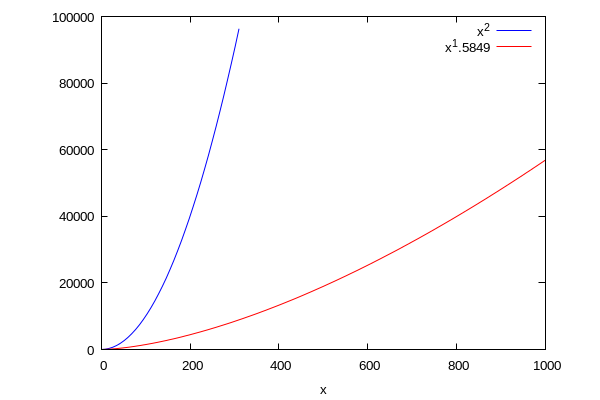
\includegraphics[width=0.6\linewidth]{comparaison2}
    \caption{Comparaison des croissances quadratique et en $n^{1.58}$}
    \label{fig:comparaison}
\end{figure}

\subsection{Compléments : représentation de la compléxité}

Nous allons illustré la complexité en temps de cet algorithme d'une façon moins classique. Dans le cas d'un calcul normal mais récursif nous devons effectuer 4 multiplications et avec l'algorithme de \textbf{karatsuba} on n'en fait que 3.

\newcommand{\carre}[2]{
    \begin{scope}[shift={#2}]
        \draw[color=black!70,fill=black] (0,0) rectangle (#1,#1);
        \draw[color=black!70,fill=black, shift={(#1,#1))}] (0,0) rectangle (#1,#1);
        \draw[color=black!70,fill=black, shift={(#1,0)}] (0,0) rectangle (#1,#1);
        \draw[color=black!70,fill=black, shift={(0,#1)}] (0,0) rectangle (#1,#1);
    \end{scope}
}
\newcommand{\kara}[2]{
    \begin{scope}[shift={#2}]
        \draw[color=black!70,fill=black] (0,0) rectangle (#1,#1);
        \draw[color=black!70,fill=white, shift={(#1,#1))}] (0,0) rectangle (#1,#1);
        \draw[color=black!70,fill=black, shift={(#1,0)}] (0,0) rectangle (#1,#1);
        \draw[color=black!70,fill=black, shift={(0,#1)}] (0,0) rectangle (#1,#1);
    \end{scope}
}
\newcount\sierpinskiorder
\newcommand\sierpinskicarpet[2][]{%
    \tikzset{sierpinski/.cd,#1}%
    \sierpinskiorder=#2\relax%
    \path [color=black!70, sierpinski/background/.try] (0,0) rectangle (1,1);
    \SierpinskiCarpet}
\def\SierpinskiCarpet{{%
        \ifnum\sierpinskiorder>0\relax
        \path [color=black!70, sierpinski/foreground/.try] (1/2, 1/2) rectangle ++(1/2, 1/2);
        \advance\sierpinskiorder by -1\relax
        \foreach \x in {0,...,1}{\foreach \y in {0,...,1}{
                \begin{scope}[shift={(\x/2,\y/2)},scale=1/2]
                    \SierpinskiCarpet
                \end{scope}
        }}
        \fi
    }
}

\begin{tabular}{|c|c|c|c|c|c|}
    \hline 
   Profondeur de récursivité & 1  &  2 & 3 & ... & $n$\\ 
    \hline 
   Algorithme classique  
  & \begin{tikzpicture}
  \carre{1}{(0,0)}
  \end{tikzpicture} 
  & 
  \begin{tikzpicture}
  \carre{0.5}{(0,0)}
  \carre{0.5}{(0,1)}
  \carre{0.5}{(1,0)}
  \carre{0.5}{(1,1)}
  \end{tikzpicture}
  & 
  \begin{tikzpicture}
 \foreach \x in {0,...,7}{\foreach \y in {0,...,7}{
         \begin{scope}[shift={(\x/4,\y/4)}]
           \draw[color=black!70,fill=black] (0,0) rectangle (0.25,0.25);
         \end{scope}
 }}
  \end{tikzpicture}
  &
  &
    \begin{tikzpicture}
  \foreach \x in {0,...,15}{\foreach \y in {0,...,15}{
          \begin{scope}[shift={(\x/8,\y/8)}]
          \draw[color=black!70,fill=black] (0,0) rectangle (0.125,0.125);
          \end{scope}
  }}
  \end{tikzpicture}
\\ 
    \hline 
Algorithme \textbf{karatsuba} &   \begin{tikzpicture}
\kara{1}{(0,0)}
\end{tikzpicture}
     &\begin{tikzpicture}
     \kara{0.5}{(0,0)}
     \kara{0.5}{(0,1)}
     \kara{0.5}{(1,0)}
     \draw[color=black!70,fill=white, shift={(1,1))}] (0,0) rectangle (1,1);
     \end{tikzpicture}  &
     \begin{tikzpicture}[scale=2]
\sierpinskicarpet[foreground/.style={fill=white},
background/.style={top color=black, bottom color=black}]{3}
\end{tikzpicture}
     &
     &
     \begin{tikzpicture}[scale=2]
     \sierpinskicarpet[foreground/.style={fill=white},
     background/.style={top color=black, bottom color=black}]{5}
     \end{tikzpicture}
     \\ 
    \hline 
\end{tabular} 

Idée prise sur \url{http://math.univ-lyon1.fr/~roblot/resources/ens_partie_2.pdf}

La courbe limite est une fractale, qui ressemble au  triangle de Serpinski. \\Pour les courbes fractales, on peut définir une dimension  \href{https://fr.wikipedia.org/wiki/Dimension_de_Hausdorff}{celle de Hausdorff}. Et le calcul de cette dimension pour notre fractale est étonnamment  $\log_2{3}=\dfrac{\ln 3}{\ln 2}$ à rapprocher de la complexité en temps de notre algorithme  $O(n^{\log_2{3}})$ .
%\subsection{Complexité en espace}
%
%Un algorithme récursif peut prendre un espace en mémoire conséquent lors de ces appels successifs. Nous allons étudier dans cette partie la taille maximale prise en mémoire par cet algorithme. 
%
%
%Nous considérons au départ deux entiers naturels non nuls $a$ et $b$ de longueur $n$ dans l'écriture décimale (c'est à dire $n=\left\lceil \log(a) \right\rceil +1$)
%\begin{propriete}
%    La profondeur maximale de l'arbre représentant les appels récursifs de cet algorithme est: \[ m=\left\lceil \log_2 n\right\rceil  - 1  \]
% \end{propriete}
%\begin{proof}
%    Le calcul est immédiat puisqu'on divise la taille $n$ de l'entier $a$  par 2 à chaque appel récursif.
% \end{proof}
%
%Pour que l'algorithme puisse s'exécuter, il doit conserver tous les appels à la fonction avec \textbf{une pile d'exécution} qui doivent contenir \[\sum_{i=0}^{m} 3^i =\dfrac{3^{m+1}-1}{2}=\Theta\left( 3^m\right) =\Theta\left( 3^{\log_2 n}\right) =\Theta\left( n^{\log_2 3}\right) \]


\section{Optimalité du problème}

La solution proposé par Karatsuba en 1962 a été la première avec une complexité sous quadratique. Une généralisation de cet algorithme a été proposé par Toom-Cook en 1963.

Pour comprendre cette généralisation revenons sur l'algorithme \textbf{Karastuba}, et en répondant à la question comment trouver le terme central en économisant le nombre de multiplication. Nous utilisons les notations de la première partie:
\begin{equation}
m(x)\x p(x) = \left( a_1 x + a_0 \right) \x \left( b_1 x + b_0 \right) = p_2 x^2 + p_1 x+ p_0
\end{equation}
Le résultat de la multiplication est un polynôme en $x$, et nous allons prendre des valeurs particulières pour trouver le résultat.
\begin{itemize}
    \item Avec le coefficient dominant, on obtient $a_1\times b_1 = p_2$
    \item Avec $x=0$, on obtient t $a_0 \times b_0 = p_0$
    \item Avec $x=-1$, on obtient $\left( a_1 -  a_0 \right) \x \left( b_1 -  b_0 \right) = p_2-p_1+p_0$ et donc \[p_1=p_2+p_0-\left( a_1 -  a_0 \right) \x \left( b_1 -  b_0 \right)\]
\end{itemize}
On retrouve le résultat de la première partie.
\subsection{Aperçu de l'algorithme de Tom-Cook}
Tom-Cook utilise cette idée en décomposant chacun des nombres en trois parties $m(x)=\left(a_2 x^2+ a_1 x + a_0 \right) $  et $p(x)=\left(b_2 x^2+ b_1 x + b_0 \right)$.  Le résultat est $p(x)=\sum_{i=0}^{4}p_i x^i$.
En évaluant le système avec le terme dominant puis la valeur en 2, 1, -1 et 0, on obtient un système d'équations qui est 
\[
 \begin{pmatrix}
 p(\infty)\\
 p(2)\\
 p(1)\\
 p(-1)\\
 p(0)
 \end{pmatrix}
  = \begin{pmatrix}
1 & 0 & 0 & 0 & 0 \\
16 & 8 & 4 & 2 & 1 \\
1 & 1 & 1 & 1 & 1 \\
1 & -1 & 1 & -1 & 1 \\
0 & 0 & 0 & 0 &  1 
\end{pmatrix}  \begin{pmatrix}
p_4\\
p_3\\
p_2\\
p_1\\
p_0\\
\end{pmatrix}
\]
Maintenant on utilise le fait que $p(x)=a(x)b(x)$ et que la matrice carrée $A$ qui est présente est inversible\footnote{$\det(A)=-12$ et $A^{-1}=\begin{pmatrix}
    1 & 0 & 0 & 0 & 0 \\
    -2& \frac{1}{6} & -\frac12 & -\frac16  & \frac12  \\
    -1 & 0 & \frac12  & \frac12  & -1 \\
    2 & -\frac16  & 1 & -\frac13  & -\frac12  \\
    0 & 0 & 0 & 0 &  1 
    \end{pmatrix}$}  , pour obtenir :
\[
 \begin{pmatrix}
p_4\\
p_3\\
p_2\\
p_1\\
p_0\\
\end{pmatrix}= \begin{pmatrix}
1 & 0 & 0 & 0 & 0 \\
16 & 8 & 4 & 2 & 1 \\
1 & 1 & 1 & 1 & 1 \\
1 & -1 & 1 & -1 & 1 \\
0 & 0 & 0 & 0 &  1 
\end{pmatrix}^{-1}  \begin{pmatrix}
a(\infty)b(\infty)\\
a(2)b(2)\\
a(1)b(1)\\
a(-1)b(-1)\\
a(0)b(0)\\
\end{pmatrix}
  \] 
 Nous avons donc 5 multiplications\footnote{on ne compte que les multiplications entre grand nombre, la multiplication par 2 ou 4 est un décalage de bit lors de l'implémentation de l'algorithme.} pour trouver la valeur du produit de $m\times p$.
 \begin{remarque}
     D'un point de vue algorithmique on aura un algorithme récursif sous forme d'arbre avec pour chaque nœud, 5 branches et comme on divise la taille du nombre de départ par 3, une profondeur de l'ordre de $\log_3(n)$.
 \end{remarque}
 \begin{propriete}
     L'algorithme de Tom-Cook a une complexité qui vérifie $ T(n)=5T\left( \dfrac{n}{3}\right) + \Theta(n) $ et donc est en $O\left( n^{\log_3 5}\right) $.
  \end{propriete}
Comme $\log_2 3 >\log_3 5$, l'algorithme de \textbf{Karatsuba} n'est pas optimal.

\subsection{Dernières avancées}
Début de cette année 2019, des chercheru

\newpage

\section*{Annexe}
\subsection*{Algorihtme pour la base binaire}
\begin{center}
    \begin{minipage}{10cm}
        \begin{algorithm}[H]
            \caption{\textbf{Fonction} karatsuba(a, b)}
            \uSi{(a < 2 ou (b < 2)}{
                \Retour{ a*b}
            }
            \vspace{1em}
            
            $m  \gets  \left\lceil \dfrac{min\left( \log(a+0.5), \log(b+0.5)\right) }{2}  \right\rceil$\;
            
            $a_1,a_2 \gets decompose(a, m)$ \;
            $b_1, b_2 \gets  decompose(b, m)$ \;
            
            $\epsilon = signe(a_2-a_1)\x signe(b_2-b_1)$\;
            $R1  \gets $ karatsuba($a_1,b_1$) \;
            $R2 \gets  $ karatsuba($a_2,b_2$)\;
            $R3  \gets $ karatsuba($|a_2-a_1|,|b_2-b_1|$)\;
            
            
            \Retour{ $R1 << {2\times m } + (R1+R2-\epsilon \x R3 ) <<  { m} + R2$}
            
        \end{algorithm}
    \end{minipage}
\end{center}
\end{document}

